%\bibliography{/home/jorgsk/phdproject/bibtex/jorgsk}
Transcription is the synthesis of a complementary RNA molecule from a DNA
template. The macromolecule that performs transcription is the DNA-dependent
RNA polymerase (RNAP). See Figure \ref{fig:transcription_elongation} for an
overview of transcription elongation by RNA polymerase.

\begin{figure}[htb]
    \begin{center}
        \includegraphics[scale=0.6]{illustrations/sysbio/1_normal_transcription.pdf}
    \end{center}
    \caption{Transcription elongation by RNA polymerase. The nascent RNA
    transcript grows at the 3\protect\ppp end where NTP binds and is
    incorporated into the RNA nucleotide chain. NTP binds in a complementary
    fashion to bases on the single stranded template DNA which are exposed due
    to the $\sim$ 14/15 bp DNA transcription bubble.}
    \label{fig:transcription_elongation}
\end{figure}

In bacteria, RNAP consists of the subunits $\beta$, $\beta^{\prime}$, $\omega$,
and two $\alpha$ subunits and has a molecular mass of around 400 kDa. The
bacterial RNAP is conserved in structure and function with RNAP found in in
archaea and eukaryotes \cite{borukhov_rna_2008}, showing that the fundamental
mechanism of RNA synthesis is the same for all cell types.

Here, we will review the role of RNAP in initiation, elongation, and
termination of transcription in bacteria. Special care will be given to the
topic of abortive transcription initiation and how RNAP moves along DNA during
transcription.

\subsubsection{Promoter localization}
Before RNAP can start transcription of a gene it must localize a transcription
start site (TSS). These sites are advertised by promoter elements, which
typically stretch from around -60 to +20 basepairs relative to the TSS
\cite{ross_third_1993,lilian_m_promoter_2002}. RNAP cannot bind strongly to the
promoters directly, but must first associate with a regulatory protein called
sigma ($\sigma$) factor; the $\sigma$ factor in turn only binds strongly to
promoters when in complex with with RNAP \cite{paget_$sigma^70$_2003}, making
the RNAP-$\sigma$ complex essential for transcription initiation. In
\textit{E.\ coli} there are seven types of $\sigma$ factors, where each
$\sigma$ factor regulates the binding of RNAP to a particular gene family
\cite{osterberg_regulation_2011}. For example, $\sigma^{70}$ recognizes
promoters for housekeeping genes, while $\sigma^{32}$ recognizes promoters for
genes that are activated in conditions of heat shock. Most promoters are of the
$\sigma^{70}$ type (meaning that $\sigma^{70}$ binds to them), and we will here
focus on this type of promoter. The most prominent $\sigma$-binding elements in
$\sigma^{70}$ promoters are the -35 and -10 hexamer (six-nucleotide) motifs,
with the consensus sequences TTGACA (-35) and TATAAT (-10)
\cite{ross_analysis_2009}. The major determinant for how strongly $\sigma^{70}$
binds to a promoter is how much the -35 and -10 motifs vary from the consensus,
as well and the distance in nucleotides between these elements. A third
sequence that affects RNAP-$\sigma^{70}$ binding is an AT rich element upstream
-35 called, simply, the upstream element \cite{ross_third_1993,
haugen_fine_2008} (see Figure \ref{fig:promoter}). In general, the stronger
$\sigma^{70}$ binds to a promoter the higher the transcription initiation rate
will be, which again tends to lead to higher expression of the downstream gene.
However, we will shortly see that the initial transcribed sequence, defined
from +1 to +20 (Figure \ref{fig:promoter}), may also influence the expression
from a promoter.

\begin{figure}[htb]
	\begin{center}
		\includegraphics[scale=0.5]{illustrations/promoter_its.pdf}
	\end{center}
	\caption{RNAP and sigma bound to promoter elements. Positions along the DNA
	template are indicated relative to the transcription start site.}
	\label{fig:promoter}
\end{figure}

\subsubsection{Transcription initiation}
% nucleotide = base-sugar-phosphate (1 or 3)
% nucleoside = base-sugar
% BUT! this confusing terminology exists: ``nucleotide with 3 phosphates'' =
% nucleoside triphosphate.
Once the RNAP-$\sigma$ complex has bound to a promoter, transcription
initiation may commence. First, $\sigma$ mediates the opening of the double
stranded DNA from -11 to +2 \cite{borukhov_rna_2008}. The unwound DNA helix is
referred to as the DNA bubble, or the transcription bubble. Within the DNA
bubble, bases on the template DNA strand are exposed and ready to base pair
with incoming NTP. After having opened the DNA bubble, RNAP is positioned so that the
nucleotide at the TSS is at RNAP's active site (the active site is the part of
RNAP where RNA synthesis occurs).  When transcription begins, the two first
nucleotides bind in the active site and a phosphodiester bond is formed between
them \cite{mcclure_steady_1978}. This constitutes the first dinucleotide of
the nascent RNA. In order to incorporate the third nucleotide, RNAP must first
move its active site relative to downstream DNA to make room for the incoming
NTP. However, RNAP is bound to the promoter, making it immobile. It can
therefore not translocate downstream as it would during transcription
elongation. Instead, translocation during initiation results in RNAP pulling
DNA into itself in a process that has been labeled ``scrunching''
\cite{kapanidis_initial_2006, revyakin_abortive_2006}.  By pulling in
downstream DNA, RNAP's active site translocates relative to template DNA,
thereby making the active site available for incoming NTP despite RNAP being
bound to the upstream promoter sequence. A consequence of scrunching is that
the DNA bubble increases in size with 1bp for each scrunching step, since one
basepair of DNA is opened downstream without the complementary closing of an
upstream basepair as for transcription elongation. The increasingly large DNA
bubble that results from scrunching has been suggested to play a role for both
promoter escape and abortive RNA release \cite{lilian_m_promoter_2002,
kapanidis_initial_2006}.

Transcription initiation proceeds in a cycle of scrunching, NTP binding, and
phosphodiester bond formation. With each step, the DNA bubble grows with one
basepair and the nascent RNA grows with one nucleotide. When the nascent RNA
reaches a length of around 10-12 nt, promoter escape may occur of $\sigma$
dissociates from the promoter \cite{lilian_m_promoter_2002} (see
Figure \ref{fig:simple_escape}).

\begin{figure}[htb]
	\begin{center}
		\includegraphics[scale=0.5]{illustrations/sysbio/7_transcription_initiation.pdf}
	\end{center}
	\caption{Promoter escape involves scrunching of DNA within RNAP.}
	\label{fig:simple_escape}
\end{figure}

\subsubsection{Abortive initiation}
Promoter escape is, however, only one outcome of a transcription initiation
attempt. Another outcome is that the initiation attempt fails, which means that
the nascent RNA is released prematurely before promoter escape can occur. The
starting point of a failed initiation attempt is a reversal of the
translocation-scrunching reaction, a step which is referred to as backtracking.
When backtracking occurs, the ``unschrunching`` of DNA forces the 3\ppp end of
the nascent RNA into the entry channel for NTP, leading to a shortened RNA-DNA
hybrid \cite{hsu_initial_2006}. This shortened RNA-DNA hybrid is unstable and
eventually the nascent RNA is released. RNA release is accompanied by a release
of the rest of the scrunched DNA from RNAP. RNAP then falls back to the open
complex formation, where it may restart transcription initiation \textit{de
novo} \cite{lilian_m_promoter_2002} (see Figure \ref{fig:abortive_backtrack}).

\begin{figure}[htb]
	\begin{center}
		\includegraphics[scale=0.5]{illustrations/sysbio/8_transcription_initiation_backtracking.pdf}
	\end{center}
	\caption{Abortive initiation caused by a backtracking-``unscrunching''
	reaction.}
	\label{fig:abortive_backtrack}
\end{figure}

The term for unscrunching and RNA release during transcription initiation is
abortive initiation. A related term is abortive cycling, which refers to
repeated initiation attempts that end with abortive RNA release (see Figure
\ref{fig:abortive_cycling}). The aborted RNA fragments are generally no longer
than 15 nucleotides, but lengths up to 20 have been observed
\cite{chander_alternate_2007}. In \textit{in vitro} experiments abortive
initiation is the rule rather than the exception \cite{lilian_m_promoter_2002}.
Some promoters have a calculated \textit{in vitro} ratio of aborted to
successful transcription initiation attempts of over 300
\cite{hsu_initial_2006}. This indicates that RNAP may on average spend
considerable time in abortive cycling before achieving promoter escape.

\begin{figure}[htb]
	\begin{center}
		\includegraphics[scale=0.4]{illustrations/sysbio/9_abortive_cycling.pdf}
	\end{center}
	\caption{Repeated abortive RNA release and \textit{de novo} transcription
	initiation is called abortive cycling.}
	\label{fig:abortive_cycling}
\end{figure}

\subsubsection{Promoter escape and the initial transcribed sequence}
An early discovery by Kammerer et al.\ \cite{kammerer_functional_1986} was that
the promoter sequence downstream +1 can have a strong effect on promoter
strength.  Kammerer et al.\ found this effect by comparing the promoter
strength of the N25 promoter with a variant of N25 constructed by changing C
for A, T for G and vice versa for N25's +1 to +20 sequence. This variant was
called N25/anti, and has later been referred to as N25$_{\text{anti}}$
\cite{,hsu_vitro_2003}.  Later, it was found that the cause for the difference
in promoter strength was a due to a large increase in the amount and the length
of abortive transcripts produced from N25/anti compared to N25
\cite{hsu_escherichia_1995, hsu_vitro_2003}. To comprehensively map the effect
of the +1 to +20 sequence on promoter escape, Hsu et al.\
\cite{hsu_initial_2006} investigated \textit{in vitro} the abortive properties
of a comprehensive library of 43 promoter variants which had randomized +1 to
+20 initial transcribed sequences (ITSs).  They showed that the sequence
variation in the ITS could result in a 20-fold difference in promoter escape
efficiencies. In the study by Hsu et al.\, the promoter escape efficiency is
defined as the fraction of full length transcript to the total amount of
transcript (full length and abortive) produced from a promoter; this quantity
is also referred to as the productive yield (PY).

For a while it was speculated that abortive initiation was an \textit{in vitro}
artefact. However, small abortive RNAs have recently been identified \textit{in
vivo} \cite{goldman_direct_2009}, demonstrating that this process occurs in
living cells. Following the discovery that abortive transcripts appear
\textit{in vivo}, it was not certain whether the abortive transcripts had any
cellular function or if they were merely artefacts of the transcription
initiation process. Yet in the last two years two studies have shown two
different functions of these short transcripts. In one, aborted transcripts
from the $\phi$10 promoter were found to deactivate a transcriptional
terminator hairpin \cite{lee_tiny_2010}. In the other, short abortive products
of 2 to 4 nucleotides in length were found to act as primers for the RNA
polymerase \textit{in vivo} \cite{goldman_nanornas_2011}; previously, it was
not known if RNAP, unlike the DNA polymerase, could use primers \textit{in
vivo}.

It is still not clear if abortive initiation is rate-limiting for natural
promoters \textit{in vivo}. However, \textit{in vitro} and \textit{in vivo}
experiments in \textit{E. coli} have shown that the transcription factors GreA
and GreB greatly reduce the amount of abortive initiation from the
N25$_{\text{anti}}$ promoter \cite{hsu_escherichia_1995}, which they do by
restoring backtracked RNAP to productive RNAP by cleaving the backtracked RNA
\cite{hsu_initial_2006, toulme_grea_2000}. This suggests that abortive
initiation has the potential to be rate limiting \textit{in vivo}, but that
this potential is countered by the expression of GreA/B. In support of an
\textit{in vivo} role for GreA in mitigating abortive initiation, it was found
that GreA resolves promoter-proximal stalling of RNAP
\cite{kusuya_transcription_2011}. However, more work is still needed to confirm
the precise role GreA/B play in promoter escape \textit{in vivo}.

\subsubsection{Transcription elongation}
Once the $\sigma$-promoter bonds are broken, RNAP is free to undergo processive
transcription elongation. However, even though $\sigma$ has broken contacts
with the promoter, it is still in a complex with RNAP immediately after
promoter escape. The bond between $\sigma$ and RNAP has, however, now been
weakened as the nascent RNA has displaced parts of the RNAP-$\sigma$
interactions on its way to the RNA exit channel of RNAP
\cite{mekler_structural_2002, nickels_interaction_2005}. It is thought that
$\sigma$ is released stochastically from this weakened complex, as $\sigma$ is
intermittently found retained with RNAP in far downstream sequences
\cite{mooney_sigma_2005}. Several studies have found that as a consequence of
$\sigma^{70}$ remaining bound to RNAP after promoter escape, the still-attached
$\sigma$ can rebind promoter-like elements during transcription elongation,
causing RNAP to pause in its track \cite{ring_function_1996,
kapanidis_retention_2005, raffaelle_holoenzyme_2005}. To escape from these
pauses, it has been suggested that RNAP-$\sigma$ must again undergo scrunching
as if it were bound to a promoter at a transcription start site
\cite{zhilina_structural_2012}.

Transcription elongation (Figure \ref{fig:transcription_elongation}) happens
with great processivity: RNAP can accurately transcribe tens of thousands of
nucleotides without dissociating from DNA. In spite of this processivity,
elongation does not occur at a constant rate. RNAP will reproducibly pause or
backtrack at certain sites \cite{herbert_sequence-resolved_2006}. Sometimes
this pausing or backtracking has a regulatory function, for example to allow
time for proper folding of the nascent RNA \cite{landick_regulatory_2006}.
Transcription elongation is in other words not just a mandatory step for
copying DNA to RNA, but also another stage of gene expression where regulation
may take place.

\subsubsection{Transcription termination}
Eventually, RNAP will dissociate DNA and release its RNA product. Two distinct
mechanisms have been identified for the release of RNA from RNAP. In one, the
protein Rho binds an unstructured region of the nascent RNA and moves along RNA
in the direction of RNAP until they meet at RNAP pause sites. At these pause
sites the interaction between Rho and RNAP causes the release of both RNA and
RNAP from the DNA template \cite{ciampi_rho-dependent_2006}. The
Rho-independent mechanism of termination begins by the formation of a strong
(GC-rich) RNA hairpin on the nascent RNA right outside the RNA exit channel. If
this hairpin is followed by a downstream A-rich sequence on DNA which
destabilizes the RNA-DNA hybrid, interactions between the hairpin and RNAP
cause RNAP to release its hold on the RNA. However, the details of the process
are not clear \cite{nudler_transcription_2002}.

In both cases, once RNA has been released, the affinity of RNAP to DNA is
greatly reduced and RNAP itself disengages DNA. When RNAP is released, it is
again free to associate with a $\sigma$ factor and begin transcription anew.
